% !TEX encoding = UTF-8 Unicode

\chapter*{Abstract}

$\alpha$-Shapes sind Graphen, welche benutzt werden können um Gestalten in Punktmengen zu identifizieren. Der Parameter $\alpha$ bestimmt die Güte der Darstellung einer Gestalt. $\alpha$-Shapes sind Subgraphen des Delaunay-Graphen. Schwellwerte, für welche sich eine $\alpha$-Shape ändert, werden mit Hilfe des Voronoi-Diagramms bestimmt.

Im Rahmen dieser Arbeit wurde eine HTML5-Applikation für PC und mobile Plattformen entwickelt. Sie veranschaulicht die $\alpha$-Shapes von Punktmengen und deren Konstruktion mit Hilfe von Delaunay-Graphen und Voronoi-Diagrammen. Durch die Darstellung bestimmter $\alpha$-Shapes lassen sich damit auch andere Eigenschaften von Punktmengen sowie markante Punkte bestimmen.

\chapter{Einführung}

In der Gestaltpsychologie, einer Teildisziplin der Wahrnehmungspsychologie, werden die Gestaltprinzipien erklärt (siehe \autocite{Goldstein2008}). Dies sind Regeln, welche erklären wie in der Wahrnehmung kleine Elemente zu größeren Objekten gruppiert werden. Eine solche Regel ist das Prinzip der Nähe: \begin{quote}
Dinge, die sich nahe beeinander befinden erscheinen als zusammengehörig. 
\end{quote}

Die im Artikel \emph{"`On the Shape of a Set of Points in the Plane"'} \autocite{alpha1983} vorgestellten $\alpha$-Shapes sind eine Formalisierung der Gestalt einer Punktmenge. Die Gestalt ergibt sich hierbei aus dem Prinzip der Nähe. Die $\alpha$-Shape ist eine Graphdarstellung, welche von einem Parameter $\alpha$ abhängig ist. Der Parameter $\alpha$ bestimmt welche Punkte zur Knotenmenge der $\alpha$-Shape gehören sowie zwischen welchen dieser Knoten die Kanten der $\alpha$-Shape liegen. Die Kanten der $\alpha$-Shape gruppieren die Punkte einer Punktmenge zu Gestalten.

Wie genau eine Gestalt mit einer $\alpha$-Shape nachempfunden wird, hängt von der Wahl des Parameters $\alpha$ ab. Es gibt keine Gesetzmäßigkeit zur Wahl eines "`guten"' Wertes für $\alpha$, da dies von der Wahrnehmung des Betrachters abhängig ist. Für die folgenden Beispiele wurde $\alpha$ so gewählt, dass die Figuren möglichst genau dargestellt werden.

\begin{figure}[htbp]
	\centering
	\subfloat[$\alpha$-Shape einer einfachen Punktmenge\label{fig:alpha_shape}]
		{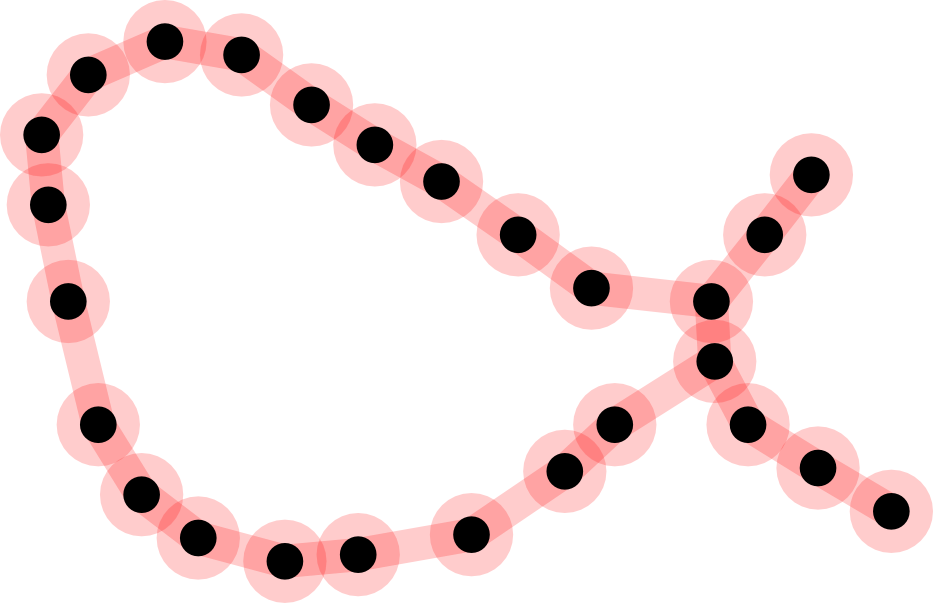
\includegraphics[scale=0.5]{../bilder/alpha_shape.png}}
	\qquad
	\subfloat[$\alpha$-Shape einer komplexen Punktmenge\label{fig:bigAS_shape}]
		{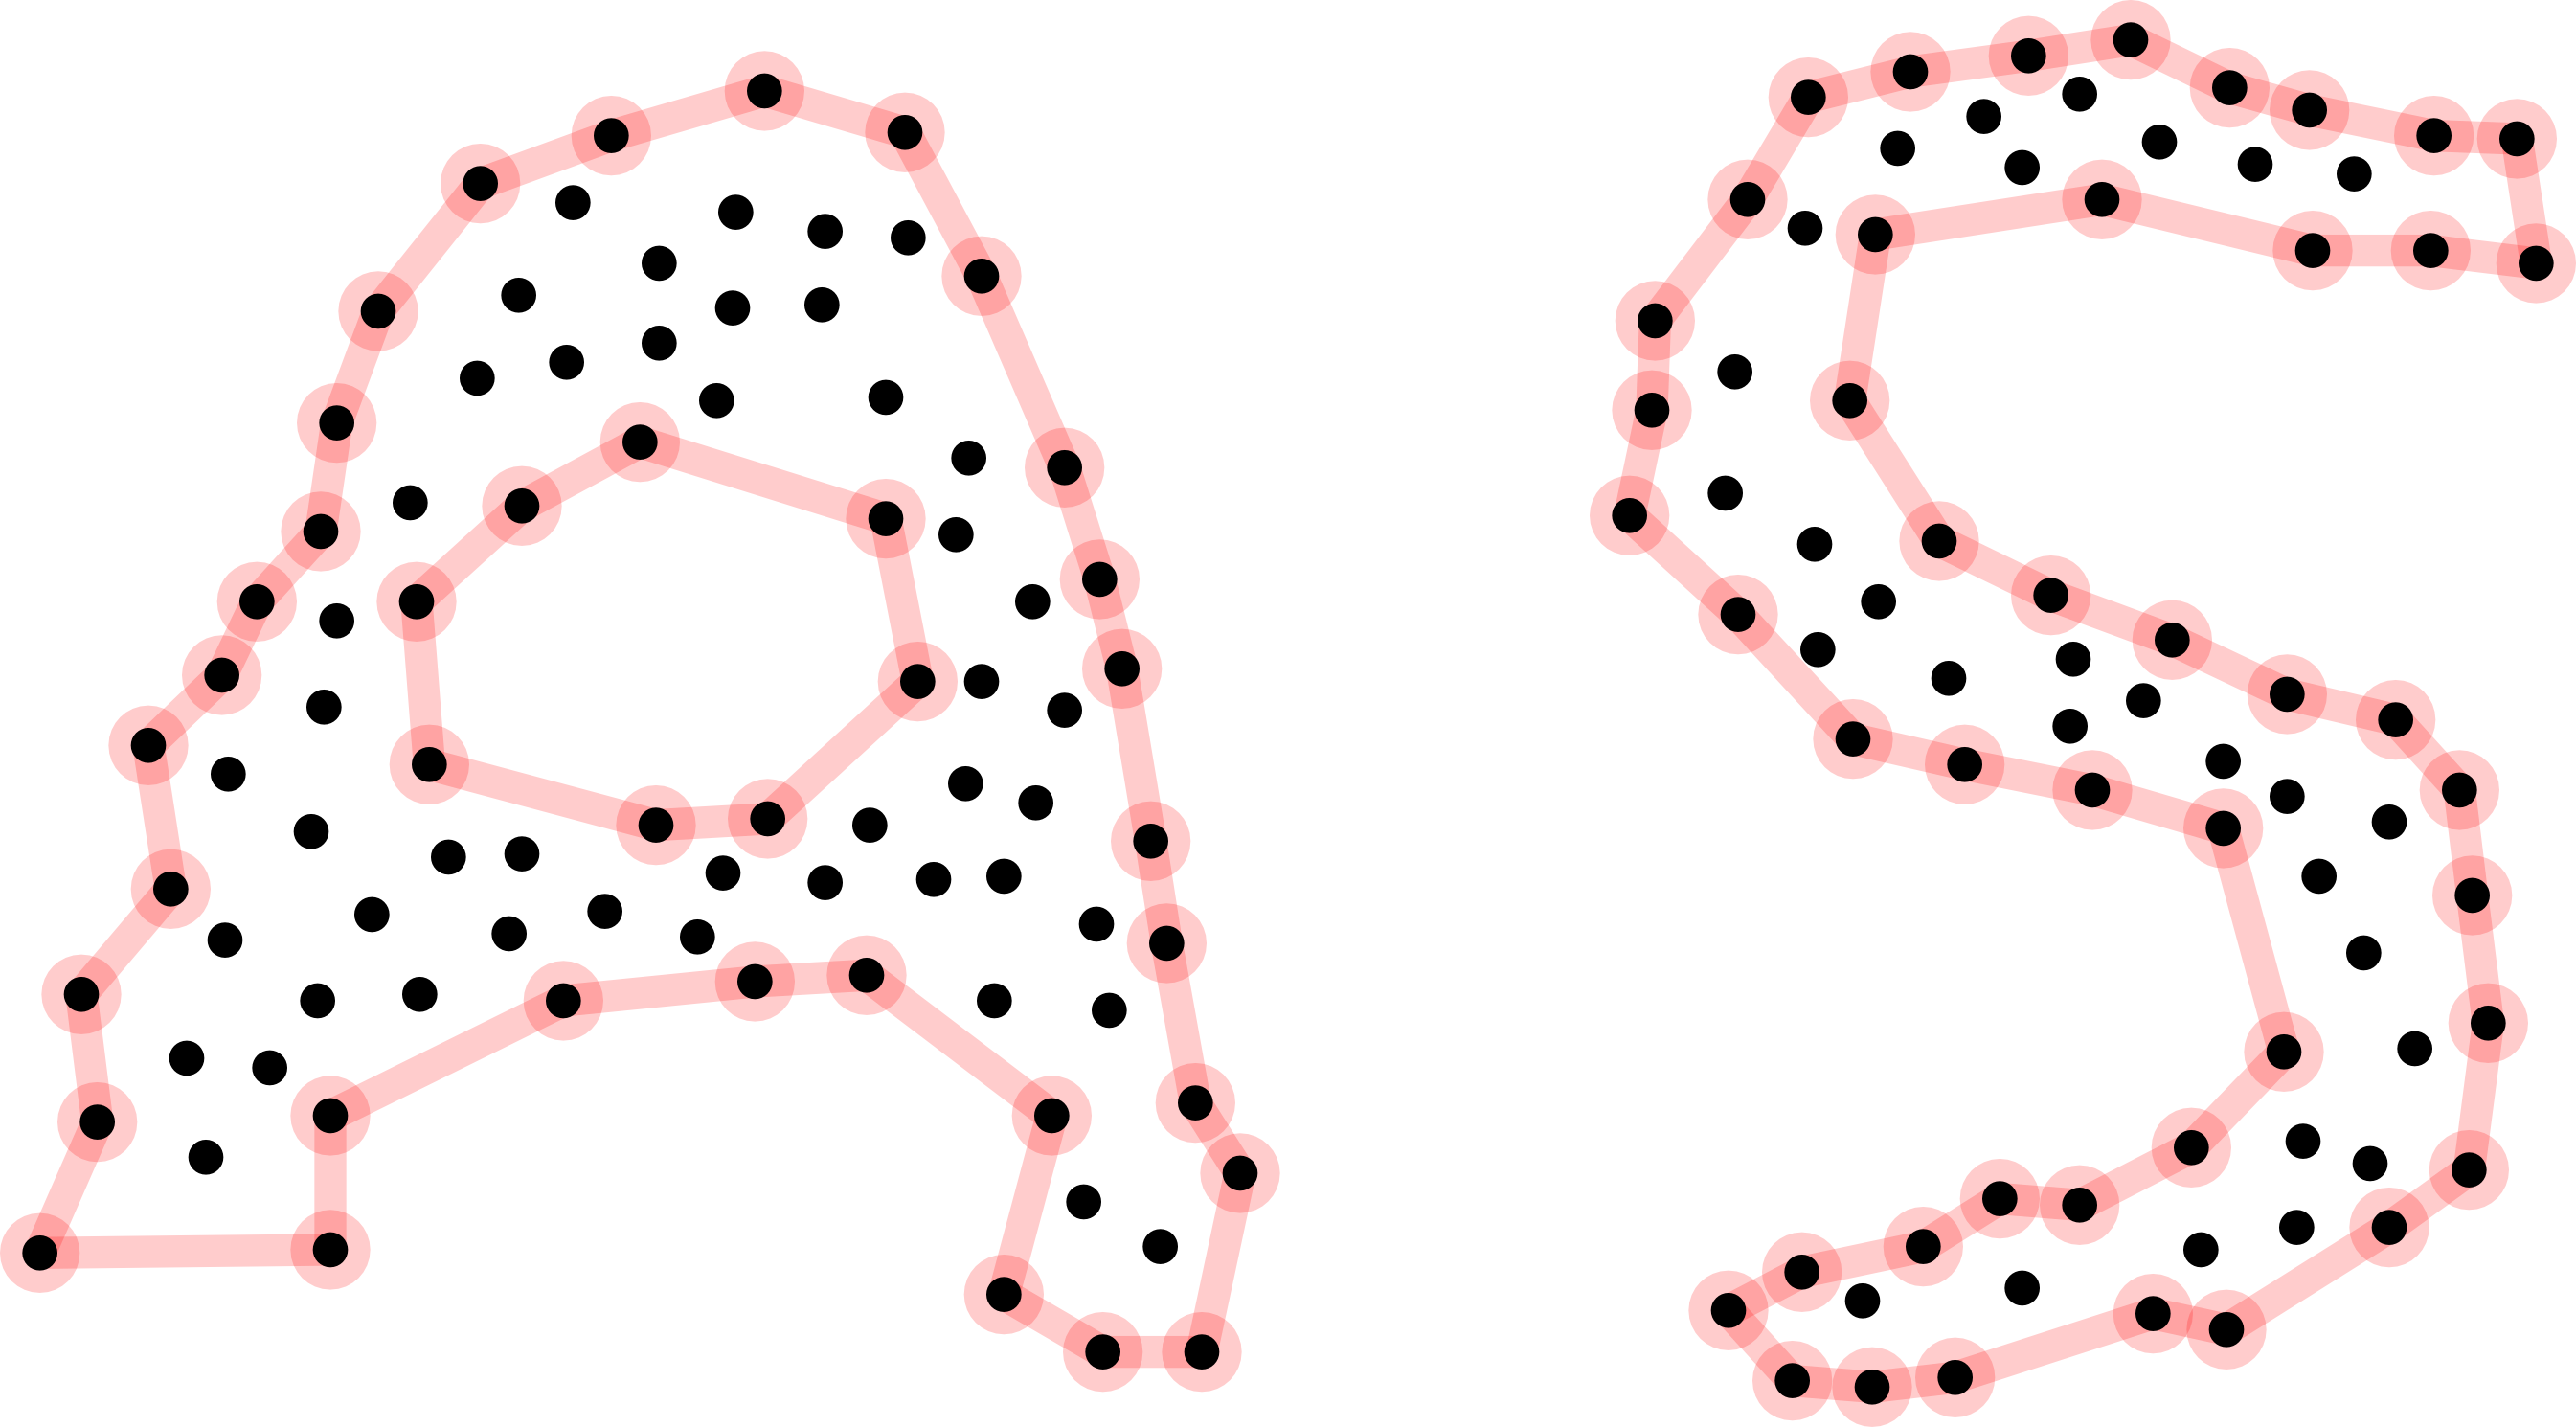
\includegraphics[scale=0.4]{../bilder/bigAS_shape.png}}
	\caption{$\alpha$-Shapes zweier Punktmengen}
	\label{fig:shapes}	
\end{figure}

In Abbildung~\ref{fig:alpha_shape} ist die $\alpha$-Shape einer einfachen Punktmenge dargestellt. Der zusammenhängende Graph verdeutlicht den Zusammenhang der einzelnen Punkte, so dass sich die Gestalt des Buchstabens $\alpha$ ergibt. In Abbildung~\ref{fig:bigAS_shape} ist die $\alpha$-Shape einer komplexen Punktmenge dargestellt. Der Graph ist nicht zusammenhängend. Die zusammenhängenden Teilgraphen begrenzen die Gestalt der Buchstaben A und S.

Die $\alpha$-Shape ist eng mit einer flächenmäßigen Darstellung der Gestalt einer Punktmenge verwandt, der $\alpha$-Hülle. Auch die $\alpha$-Hülle gruppiert Punkte nach dem Prinzip der Nähe und ist von demselben Parameter $\alpha$ abhängig.

\begin{figure}[htbp]
	\centering
	\subfloat[$\alpha$-Hülle einer einfachen Punktmenge\label{fig:alpha_hull}]
		{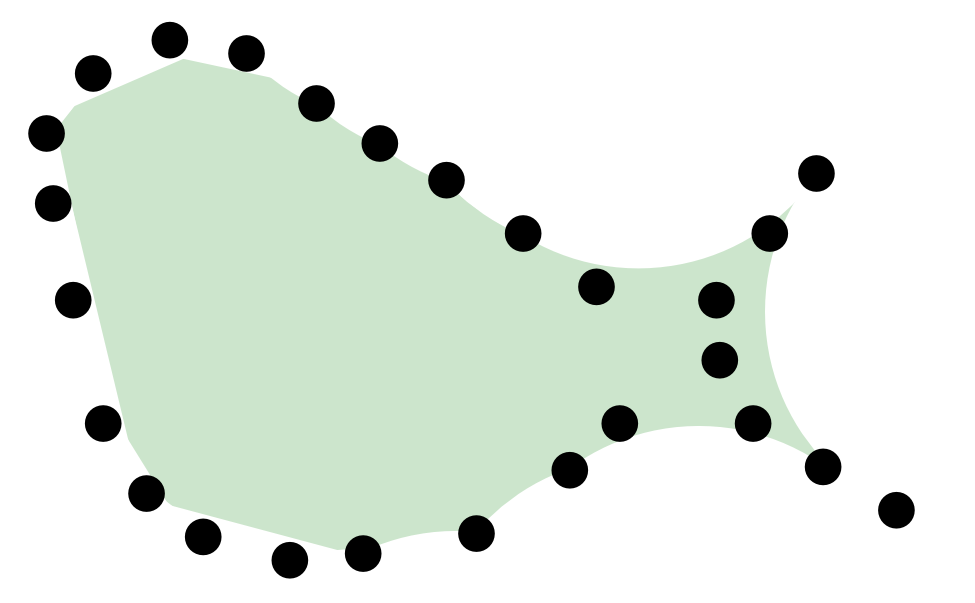
\includegraphics[scale=0.5]{../bilder/alpha_hull.png}}
	\qquad
	\subfloat[$\alpha$-Hülle einer komplexen Punktmenge\label{fig:bigAS_hull}]
		{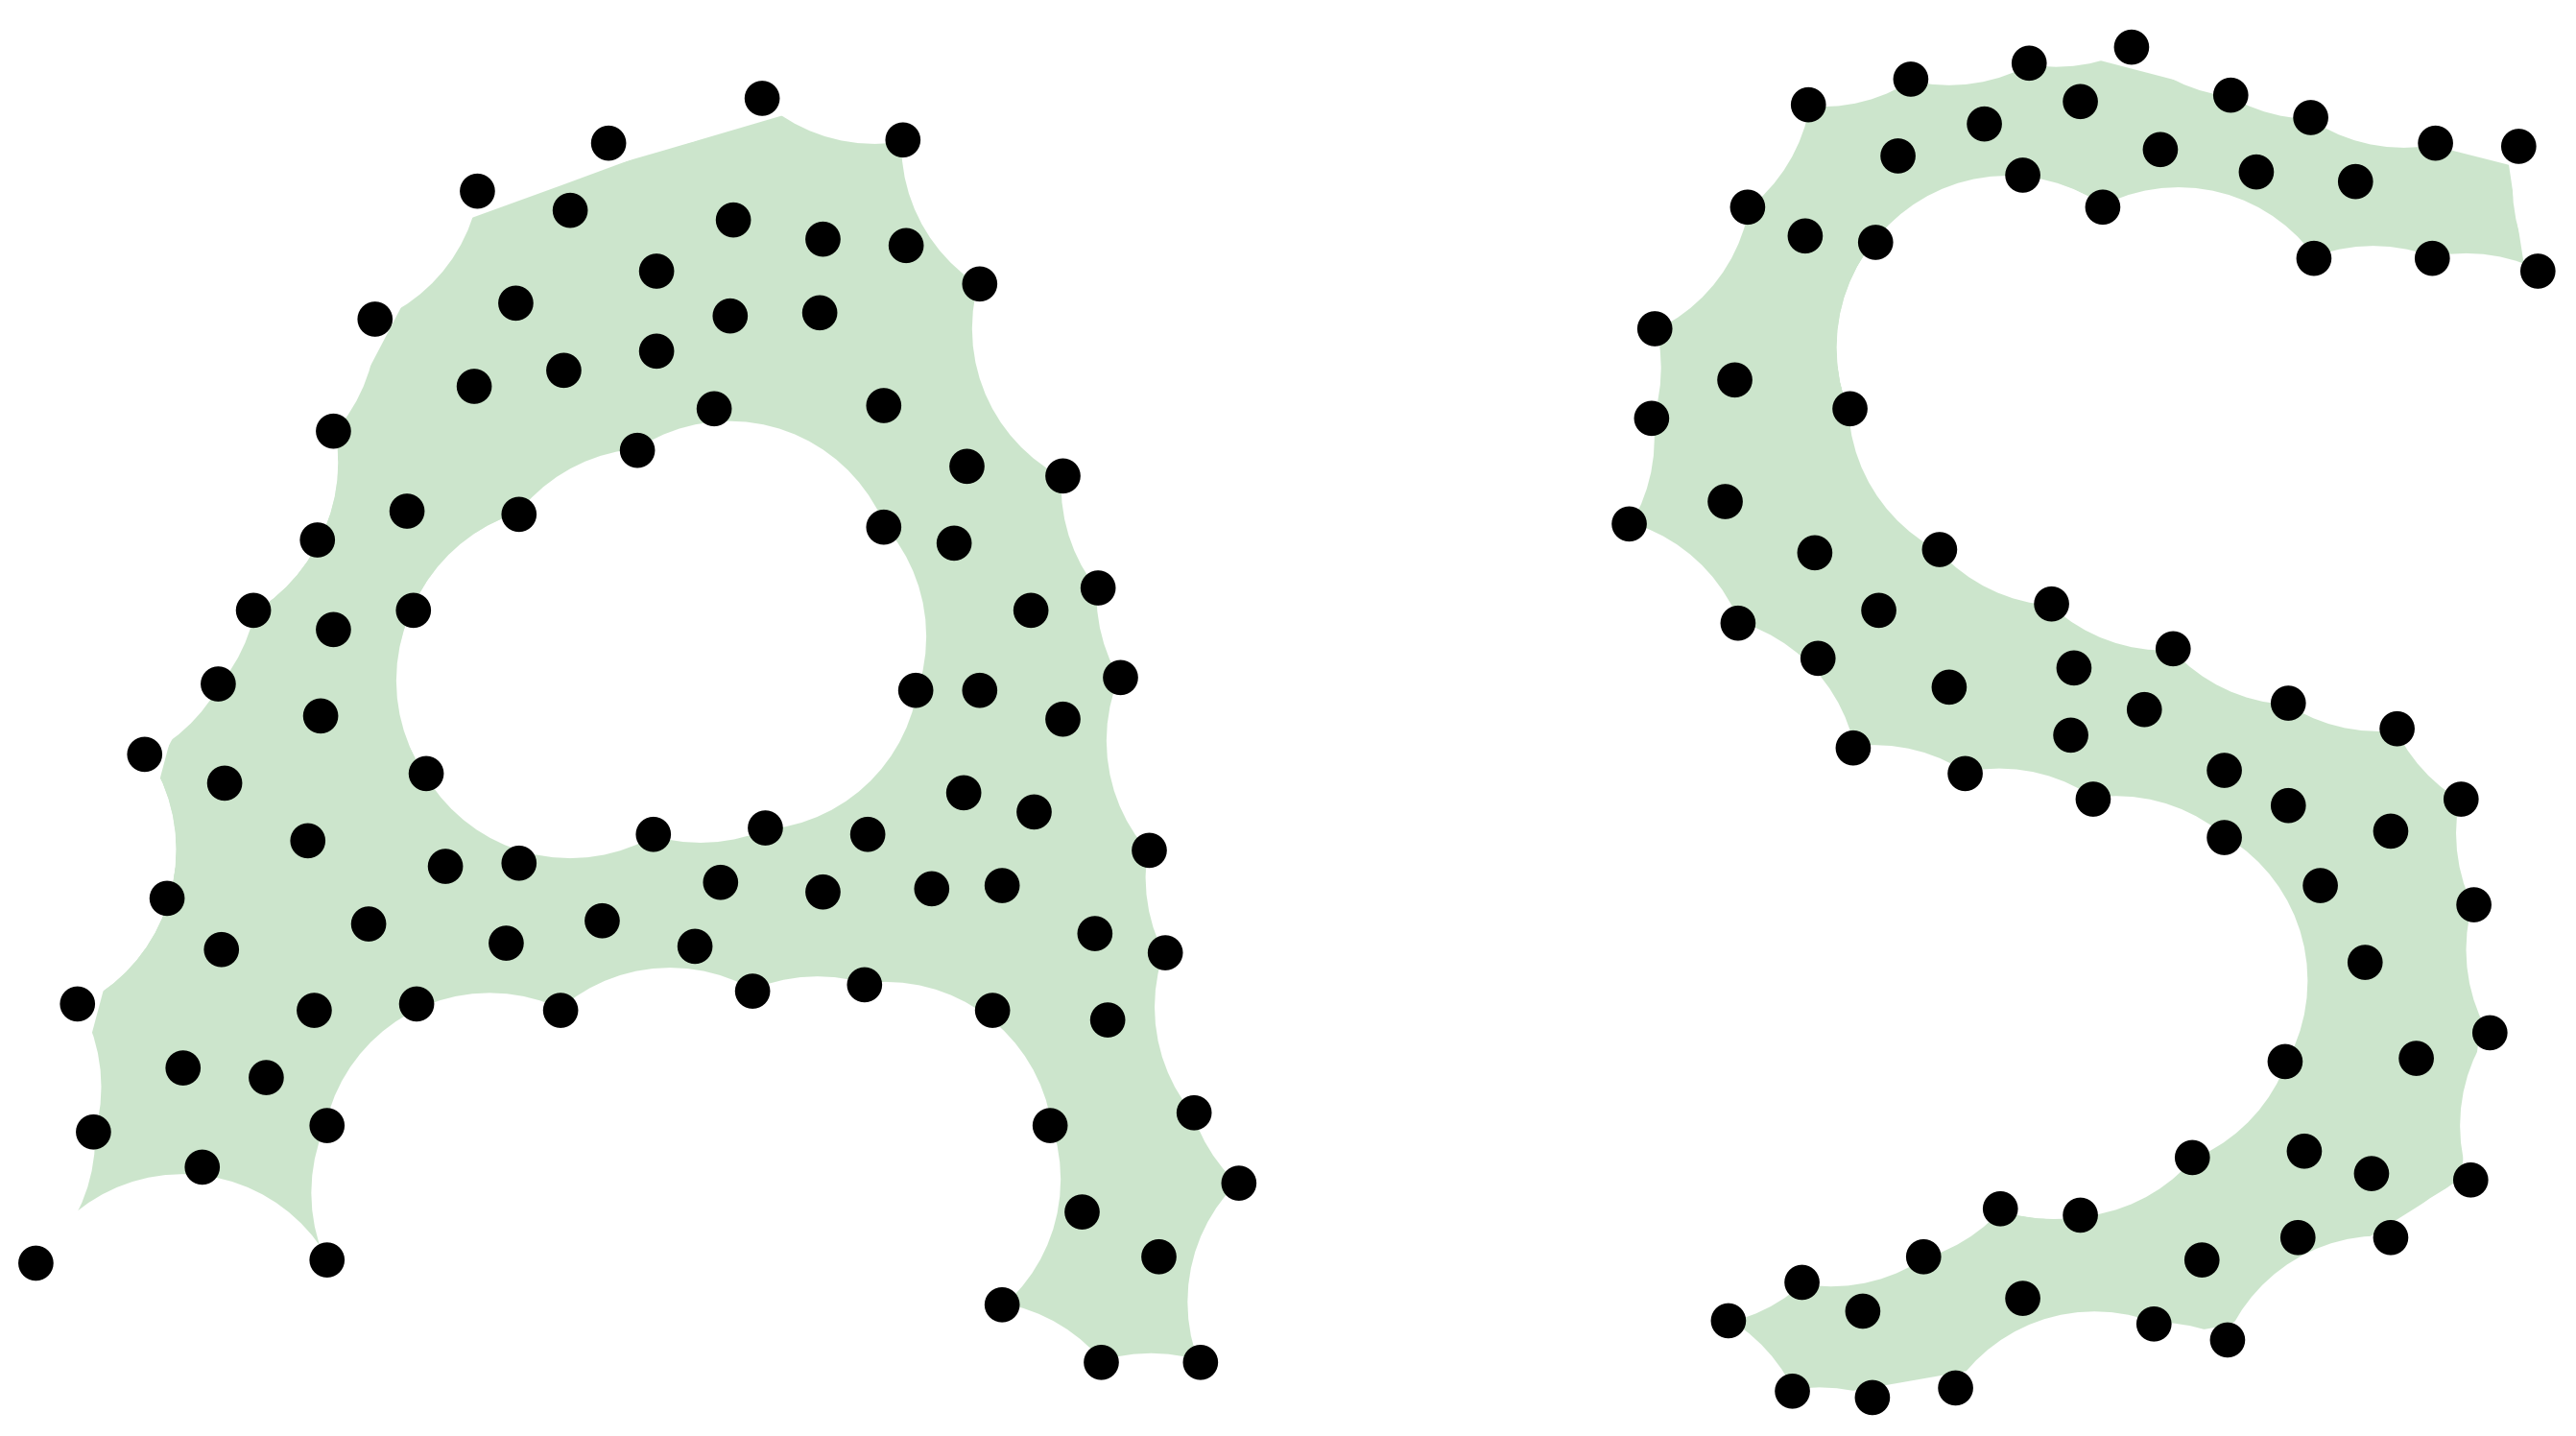
\includegraphics[scale=0.4]{../bilder/bigAS_hull.png}}
	\caption{$\alpha$-Hüllen zweier Punktmengen}
	\label{fig:hulls}	
\end{figure}

Abbildung~\ref{fig:hulls} zeigt $\alpha$-Hüllen für die Punktmengen aus Abbildung~\ref{fig:shapes}. Auch hier ist $\alpha$ wieder so gewählt worden, um eine möglichst gute Darstellung der durch die Punktmenge angenäherten Figuren zu erhalten.
